\documentclass{article}
\usepackage[utf8]{inputenc}
\usepackage{geometry}
\geometry{a4paper, margin=1in}
\usepackage{amsmath}
\usepackage{amsfonts}
\usepackage{amssymb}
\usepackage{graphicx}
\usepackage{enumitem}
\usepackage{xcolor}
\usepackage{float}
\usepackage{subcaption}
\usepackage{longtable}

\title{Project-X: Architectural Evolution - Old vs. New}
\author{Alberto Espinosa\\
KSquare Group}
\date{July 18, 2025}

\begin{document}
\maketitle

This document outlines the key changes, adaptations, and equivalences between the original Project-X architecture and the newly proposed agent-based architecture leveraging Ollama and LangGraph, updated as of 06:57 AM CST. The platform supports multiple use cases, including fraud detection, supply chain optimisation, and customer analytics.

\section{Original Architecture Overview}
The original Project-X architecture focused on distinct components for data ingestion, predictive modelling, business rule application, and a centralised decision engine, all feeding into a user interface. It laid a solid foundation for data-driven decision-making.

\begin{figure}[H]
    \centering
    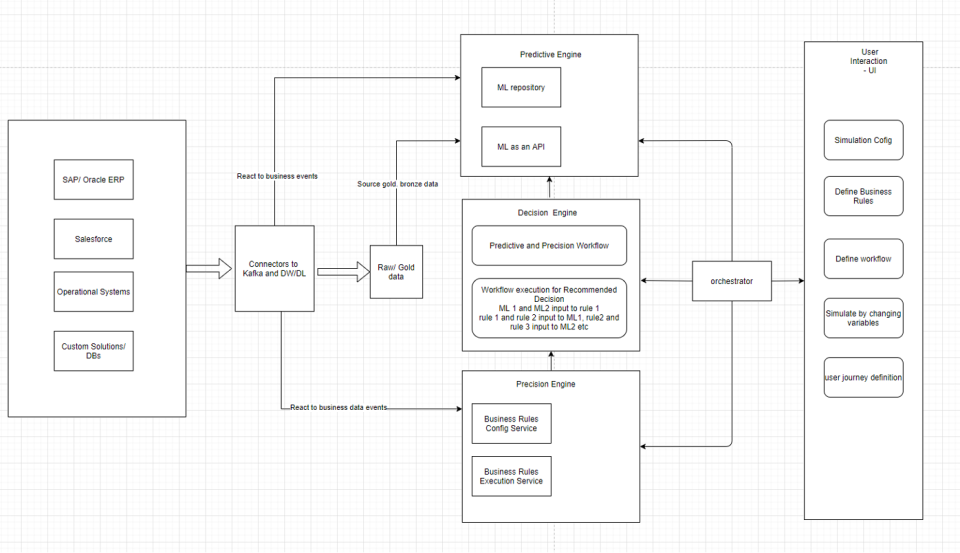
\includegraphics[width=0.9\textwidth]{ProjectX Architecture.png}
    \caption{Original Project-X Architecture Diagram}
    \label{fig:old_architecture}
\end{figure}

\section{Key Driving Principles for Adaptation}
The adaptation to an agent-based architecture is driven by the desire for:
\begin{itemize}
    \item \textbf{Enhanced Intelligence \& Adaptability:} Utilising LLMs for more nuanced understanding and dynamic behaviour.
    \item \textbf{Increased Automation:} Automating complex tasks like code generation and intelligent data handling.
    \item \textbf{Transparency \& Explainability:} Providing clear reasoning for decisions and actions.
    \item \textbf{Scalability \& Efficiency:} Leveraging LLMs for reasoning while offloading heavy computation.
    \item \textbf{Empowered User Interaction:} Enabling more intuitive configuration and understanding for business users.
\end{itemize}

\section{Architectural Changes, Adaptations, and Equivalences}

The table below details how each module from the original architecture has evolved in the agent-based design.

\begin{longtable}{|p{4cm}|p{6cm}|p{6cm}|}
    \hline
    \textbf{Original Module} & \textbf{New Agent-Based Adaptation} & \textbf{Changes/Equivalences} \\
    \hline
    \endfirsthead
    \multicolumn{3}{c}%
    {{\bfseries \tablename\ \thetable{} -- continued from previous page}} \\
    \hline
    \textbf{Original Module} & \textbf{New Agent-Based Adaptation} & \textbf{Changes/Equivalences} \\
    \hline
    \endhead
    \hline \multicolumn{3}{|r|}{{Continued on next page}} \\ \hline
    \endfoot
    \hline
    \endlastfoot

    \textbf{Data Sources} & \textbf{Data Sources} & No fundamental change in external data origin. \\
    \textit{SAPI Oracle ERP, Salesforce, Operational Systems, Custom Solutions/DBs} & \textit{SAPI Oracle ERP, Salesforce, Operational Systems, Custom Solutions/DBs} & These remain the foundational data providers (integration planned post-MVP with synthetic data focus initially). \\
    \hline

    \textbf{Connectors to Kafka and DIVIDL} & \textbf{Connectors (to Kafka and DIVIDL) \& Data Ingestion Agents (Stream Processor Agent)} & \textbf{Adaptation:} Connectors remain, but are now intelligently augmented by Data Ingestion Agents (post-MVP integration). \textbf{Validation:} Hybrid validation (rules + LLM-driven semantics) ensures data integrity across use cases. Tools: SciPy, pandas. Success metric: 98\% accuracy in routing and metadata generation. \textbf{Performance:} Stress-tested with high-throughput streams (e.g., 1000 events/second). Tools: JMeter, Locust. Metrics: Latency < 100ms, throughput > 1000 events/second. \textbf{Integration:} Post-MVP real-time integration with Kafka and DIVIDL, using exponential backoff retries, dead-letter queues, and batch processing. Metrics: Ingestion latency < 50ms, error rate < 1\%. \\
    \textit{React to business events, Raw Gold Data, Source Gold Bronze Data} & \textit{Data Ingestion Agents (Stream Processor Agent)} & \textbf{New Capabilities:} LLM-driven intelligent parsing, hybrid validation, dynamic routing, rich metadata generation, summarisation (initially with synthetic data). \\
    & \textit{Raw Gold Data, Source Gold Bronze Data} & Data output layers remain, enhanced by agent processing post-MVP. \\
    \hline

    \textbf{N/A (New)} & \textbf{Synthetic Data Generation Agent (Code Generator)} & \textbf{New Addition:} An entirely new capability for programmatically generating synthetic data for MVP across multiple use cases. \textbf{Validation:} Statistical tests (e.g., Kolmogorov-Smirnov) ensure data aligns with use case distributions. Tools: SciPy, pandas. Success metric: p-value > 0.05. Code validated via pytest (95\% pass rate). \textbf{Performance:} Tested for code generation efficiency under load. \\
    \textit{No equivalent in old architecture} & \textit{Agent generates code for data creation using libraries like Faker, SciPy.} & Addresses the need for robust test/training data, especially when real data is scarce or sensitive. \\
    \hline

    \textbf{Predictive Engine} & \textbf{Predictive Engine (AutoML Orchestration Agent)} & \textbf{Adaptation:} Enhances the model creation process with AutoML intelligence. \textbf{Validation:} Generated pipelines evaluated using cross-validation and use case-specific metrics (e.g., F1 > 0.85). Tools: PyCaret, scikit-learn. \textbf{Performance:} Tested for model inference speed under high load. \\
    \textit{ML repository, ML as an API} & \textit{ML Repository, ML as an API, AutoML Orchestration Agent} & \textbf{Changes:} The AutoML Agent (powered by Ollama) can analyse synthetic datasets and tasks to generate PyCaret code, automating model building, tuning, and evaluation. \\
    & & The ML Repository and ML as an API remain the storage and serving layers. \\
    \hline

    \textbf{Precision Engine} & \textbf{Precision Engine (Business Rule Management Agent)} & \textbf{Adaptation:} Streamlines rule definition and management. \textbf{Validation:} LLM-translated rules cross-checked against test suites for diverse use cases. Tools: Custom validation scripts. Success metric: 98\% accuracy. \textbf{Performance:} Tested for rule execution efficiency. \\
    \textit{Business Rules Config Service, Business Rules Execution Service} & \textit{Business Rules Config Service, Business Rules Execution Service, Business Rule Management Agent} & \textbf{Changes:} The Business Rule Management Agent (Ollama-powered) allows natural language input for rules, translating them to structured formats. \\
    & & The core services are retained as tools for the agent. \\
    \hline

    \textbf{Decision Engine} & \textbf{Decision Engine (LangGraph Core)} & \textbf{Fundamental Transformation:} Moves from a fixed workflow to a dynamic, intelligent agent graph. \textbf{Validation:} Explanations evaluated for clarity (90\% rated clear). Conflicts resolved without human intervention in 95\% of cases. \textbf{Performance:} Stress-tested with complex workflows (e.g., 100 concurrent decisions). Tools: Locust, Prometheus. Metrics: Latency < 100ms, throughput > 100 decisions/second. \\
    \textit{Predictive and Precision Workflow, Workflow execution for Recommended Decision} & \textit{LangGraph-Powered Orchestration, Decision Orchestration Supervisor Agent, Sub-Agents (Prediction Request, Rule Application, Data Query, Human-in-the-Loop, Conflict Resolution Agents)} & \textbf{Changes:} LangGraph defines stateful workflows with agent collaboration. Decisions use adaptive reasoning with synthetic data initially. \\
    \hline

    \textbf{Orchestrator} & \textbf{Orchestrator (API Gateway)} & \textbf{Adaptation:} Becomes primarily an API gateway to the new agentic backend. \textbf{Performance:} Tested for API routing efficiency under high request volumes. \\
    \textit{Links backend processing with UI} & \textit{Routes UI requests to LangGraph workflows, translates agent responses.} & \textbf{Changes:} Focuses on communication mediation, with workflow logic in LangGraph. \\
    \hline

    \textbf{User Interaction - UI} & \textbf{User Interface (UI)} & \textbf{Enhancement:} Becomes a more powerful interaction point. \textbf{Performance:} Tested for responsiveness under high user interaction loads. \\
    \textit{Simulation Config, Define Business Rules, Define workflow, Simulate by changing variables, user journey definition} & \textit{Simulation Config, Define Business Rules, Define Workflow (Visual LangGraph Editor), Simulate by Changing Variables, User Journey Definition, Agent Interaction Interface} & \textbf{New Capabilities:} Basic Agent Interaction Interface for MVP, with Visual LangGraph Editor planned post-MVP. \\
    \hline

\end{longtable}

\section{Roadmap Overview}
The development of the new agent-based architecture follows a structured roadmap, detailed in the separate document \texttt{project\_x\_roadmap.tex}. Key phases include MVP Development (July--August 2025), Validation (August--September 2025), Performance Testing (September--October 2025), Integration (October--November 2025), and Post-MVP Enhancements (December 2025 onward), with dependencies ensuring a phased rollout.

\section{Conclusion}
The shift to an agent-based architecture with Ollama and LangGraph transforms Project-X into a more intelligent, adaptive platform, starting with synthetic data for MVP. It leverages LLMs for reasoning and code generation, integrating existing components as tools, with plans for real-data integration post-MVP for greater flexibility and scalability across multiple use cases.

\end{document}